% !TeX TS-program = xelatex

\documentclass{resume}
\usepackage{graphicx}                                                           
\usepackage{float} 
\ResumeName{Liu Jinfan}

\begin{document}

% % TODO: Figure Insertion
% \usepackage{wrapfig}
% \begin{wrapfigure}{r}{4cm} 
%     \centering
%     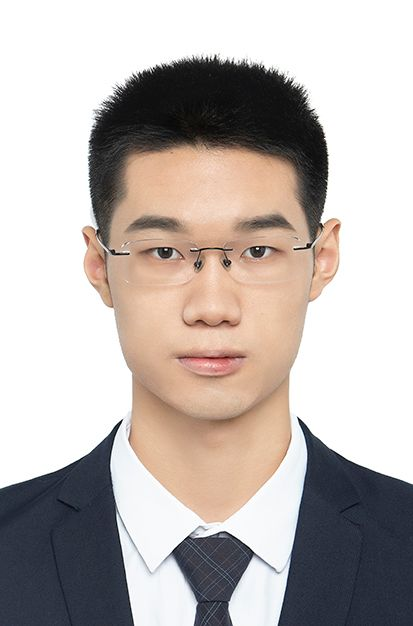
\includegraphics[width= 0.5in]{pic.png}
% \end{wrapfigure}

\ResumeContacts{
    (+86) 15008278732,%
    \ResumeUrl{mailto:3020202184@tju.edu.cn}{3020202184@tju.edu.cn},%
    \\ 
    \ResumeUrl{https://chrisvicky.github.io/}{chrisvicky.github.io} \footnote{Underlined content contains hyperlinks.},%
    \ResumeUrl{https://github.com/ChrisVicky}{github.com/ChrisVicky}%
    }

    \ResumeTitle

    \section{Education}
    \ResumeItem
    [Tianjin University (TJU)|Undergraduate]
    {Tianjin University}
    [\textnormal{Computer Science and Technology|} Undergraduate]
    [2020.09—2024.06 (Expected)]


    \section[Technical Skills]{Technical Skills\protect}
    \begin{itemize}
        \item \textbf{Programming Languages}: C/C++, Python, SQL, Java, Golang, Lua, Rust, Shell, Matlab, Tex, etc.
        \item \textbf{Workflow}: Arch Linux, Shell, (Neo)Vim, Git, GitHub, IDEA (SpringBoot), etc.
        \item \textbf{Back-End}: Java (SpringBoot), Golang (GORM), Python (Flask), SQL, Docker, Redis, nginx, WASM, etc.
        \item \textbf{Research}: Distributed Swarm Control, ROS, CV, Wi-Fi positioning, Multimodal Perception, PyTorch ML, etc.
    \end{itemize}

    \section{Project Experience}

    \ResumeItem{TJU•TWT Studio}
    [Back-end Team Leader•\ResumeUrl{https://github.com/ChrisVicky/52Hz}{“52Hz”} Development and Maintenance]
    [2021.03-2021.05] 

    \begin{itemize}
        \item \textbf{Independently completed} the redesign and implementation of the database, business logic, and core matching algorithm
        \item \textbf{Coordinated} the switch of other team developers to the new API and product testing, ensuring the project was launched on time on 520
    \end{itemize}

    \ResumeItem{TJU•TWT Studio}
    [Back-end Team Leader•“BBS” Maintenance and Refactoring]
    [2022.06 - Now] 

    \begin{itemize}
        \item \textbf{Organized} three developers to refactor “BBS (Campus Forum)” from Golang's GORM framework to Java's SpringBoot framework
        \item \textbf{Responsible for} the main maintenance work, including the design and implementation of Java and Golang patch codes and server maintenance issues
    \end{itemize}

    % \ResumeItem{TJU•Computer Network Course}
    % [\ \ResumeUrl{https://github.com/ChrisVicky/TJU-2022-Socket-Computer-Network-Lab}{Implementing a C server based on the socket interface}\footnote{Final report scored 99 points}]
    % [2022.04.14]
    %
    % \ResumeItem{TJU•Computer Network Practice}
    % [\ \ResumeUrl{https://github.com/ChrisVicky/TJU-2022-TCP-Computer-Network-Lab}{Implementing reliable TCP transmission protocol using UDP}\footnote{100 points}]
    % [2022.10.19]

    \section{Research Experience}

    \ResumeItem{Hu Qinghua Research Group}
    [\textbf{National}]
    [2021.09 - 2022.09]
    \begin{itemize}
        \item \textbf{Implemented} distributed control and synchronization of multiple quadrotor drone swarms driven by the ROS system, and the model solving local optimal solutions
        \item Hand-made and drove multiple drones, conducted flight tests and other experiments, pioneering real-machine experiments in the research group
        \item \textbf{Responsible for} organizing the research results and team "Z.E.U.S: Disaster Emergency Drone Swarm System" to participate in "Internet+" and other competitions, winning the gold medal
    \end{itemize}

    \ResumeItem{Tong Xinyu Research Group}
    [\textbf{Team Leader}]
    [2022.09 - Now]
    \begin{itemize}
        \item \textbf{Assisted} the PhD students of the research group in validating the efficiency and performance differences of LSTM in RFID system positioning prediction models in PyTorch and Matlab implementations  
        \item \textbf{In charge of} the main research, code design, and implementation of the project "Synchronization and Perception of Visual and Wi-Fi Multi-modal Maps", main technology stack: libfreenect2 open-source library, libssh, SLAM, OpenCV library, YOLOv5 model, socket framework, cURL library, Flask framework
    \end{itemize}

    % \ResumeItem{TJU•Deep Learning Course}
    % [\ \ResumeUrl{https://github.com/ChrisVicky/TJU-2023-Deep-Learning-Report/tree/main}{Improving Vision Transformer}\footnote{90 points}]
    % [2023.01.15]
    %
    % \ResumeItem{TJU•Computer Vision Course}
    % [\ \ResumeUrl{https://github.com/ChrisVicky/TJU-2023-Computer-Vision-Final}{Control Net Control Module Based on Optical Flow}\footnote{Scores not yet released}]
    % [2023.04.15]


    \section{Awards}
    \ResumeScholar{Suzhou Yuchai Scholarship (10,000 yuan)}[2022.11.15]
    \ResumeScholar{TJU 2021 Outstanding Student}[2021.10.31]
    \ResumeScholar{The Second Chuan-Shu Model Student Aid Award (60,000 yuan)}[2020.07.14]
    \ResumeScholar{NOIP (First Prize)}[2018.12.15]
    \ResumeScholar{The 31st Chengdu Youth Science and Technology Innovation Competition (Elite Award)}[2015.12.04]



    \section{Personal Summary}

    \begin{itemize}
        \item Loyal user of Arch Linux, with rich experience in software development and "tinkering", has written multithreaded programs. \textbf{English: TOEFL 104} \footnote{Test on January 14, 2023 (Reading 26, Listening 26, Speaking 25, Writing 27)}
        \item \textbf{GPA: 3.78/4.0}, participated in multiple engineering and research projects while maintaining a good GPA. Actively participated in public welfare activities to broaden horizons. Understands and studies \ResumeUrl{https://suckless.org/}{suckless} and other software design philosophies

    \end{itemize}


\end{document}
